\documentclass{article}

\usepackage[T1]{fontenc} 
\usepackage[utf8]{inputenc} 
\usepackage[UKenglish]{babel}
\usepackage{graphicx} 
\usepackage{listings} 
\usepackage[hidelinks]{hyperref}
\usepackage{enumitem} 
\usepackage{amsmath} 
\usepackage{tikz} 
\usepackage{float}
\usepackage{verbatim} 
\usepackage{xcolor}
\title{DM565 Innovation Project} 
\author{authors} 
\date{\today}

\definecolor{commentsColor}{rgb}{0.497495, 0.497587, 0.497464}
\definecolor{keywordsColor}{rgb}{0.000000, 0.000000, 0.635294}
\definecolor{stringColor}{rgb}{0.558215, 0.000000, 0.135316}

\begin{document}

\maketitle

\newpage

\tableofcontents

\newpage

\section{Introduction}
This report concerns the innovation project in the Formal Languages and Data Processing
course. The task of this project is to find an idea for a product involving some type of
open data, and then  evaluate the this idea as a
basis for a startup in a structured manner with the business model canvas.
Finally we need to construct a prototype showing the idea in practice. 
\section{Idea Description}
\begin{comment}
 we need to focus our idea, as discussed in the midwayseminar. The best is to have a core
idea that we focus on. 
\end{comment}
The basis of the idea is to  web scrape recipes of different sites, to create a database
of various recipes and the ingredients of these recipes. This database of recipes and
ingredients will then be
paired with the cost of these ingredients included in the recipe. This will enable us to
show an estimate of the cost of making the recipe. The cost of the different ingredients can be
found using the public product suggestion API made by the retail company Salling. This API
references the prices on the \url{bilkatogo.dk} website. Another resource for current
pricing information is from the \url{etilbudsavisen.dk} API, which shows the current
offers of local chains. Prices are also available on some pages that do not have any APIs.
Here is another place that we may need to use web scraping. This price information can
be used to let the users query recipes based on their specific budgets. Another way for
the product to utilize the price information, is that the user can input their current owned
ingredients, and get suggestions on  recipes of which the user is only missing a few
ingredients to be able to make. This can help combat the waste of food.


\section{Business Model Canvas}

For evaluating our idea the business model canvas will be used. The business model canvas
is a template for systematically documenting the business model of an existing business or
prospect startup. The business model canvas focuses on four different key areas of a
building a sustainable business: \begin{enumerate}[itemsep=0pt]
  \item Infrastructure
  \item Offering
  \item Customers
  \item Finances
\end{enumerate}

\subsection{Offering}
The offering is the our value proposition. The value proposition is the services that our
product provides. The value proposition is what sets the product apart from the
competition. The value which we provide to the customer, is to give the ability to view
prices of items that are in a given recipe, this will also present the total cost of the
recipe to the customer. The product will also provide value in enabling the customer to
submit their own recipes, to share with other customers. Given that we have different
recipes with price data, we can also provide the users with options for a number of
recipes given different price points. The problem we solve for the customer is the
issue of estimating the cost of a given recipe.  Another problem, which we could solve for
the customer is the issue of finding a recipe for which the user already has the
ingredients (or some subset of ingredients). Solving this problem for the customer can
also contribute to less wasted food. It is clear that different services can cater to
different customer segments.  Eg. more cost-concious consumers may be drawn to the feature
of a total cost estimate of a given recipe. The general the value proposition of our
product is to provide a service, which gets the job done, and offers convenience for the
customer. 


\subsection{Infrastructure}
\subsubsection{Key Activities}
The key activities, are the most important activities for executing our value proposition.
To provide value for our customers we examine which key activities our value proposition
requires. In our key activities we first and foremost focus on problem solving:

\begin{enumerate}
  \item To provide value in terms of offering a price estimate on recipes, we first and
    foremost must establish a system, which handles recipes and the ingredients of these
    recipes. The ingredients of the different recipes must be linked with prices of
    products.
  \item We must provide a way of presenting the recipes to the user in appealing way.
  \item Providing ways for the customer to participate in a community, thus engaging the
    customer and pushing them to share recipes and thus provide value for other customers. 
\end{enumerate}

\subsubsection{Key Resources}
Key resources are the resources, which our value propositions, distribution channels,  
customer relationships and revenue streams require. One of our key resources is the data
generated by the customers, when they submit recipes. Another key resource is the public
API provided by Salling, which aides in producing the prices of individual ingredients.
Active users is also a key resource, in that they bring in advertisement revenue. Thus it
is important to keep a good relation to customers, such that they come back for more
recipes.

\subsubsection{Key Partners}
A key partner is Salling, which provides pricing data from their open API. This pricing
data is hard to source from other places, thus they are an integral partner to our
business. A key supplier
is the hosting service, which delivers hosting for our website. A hosting service should
provide a reliable service, such that we can guarantee availability to our customers.
Another key partner is various search engines (although mostly Google), this is of utmost
importance, since the vast majority of site visits will come from people searching for a
specific recipe. Thus optimizing our service for discoverability (Search Engine
Optimization) is very important in acquiring new consumers.

Down the line we could also incorporate prospect key partners, these could be different
retail chains sharing prices with us. This could enable us to provide more value to our
customers in terms of comparing prices and enabling competition.

\subsection{Customers}
\subsubsection{Customer Segments}
At first we must examine who our customers are, in order to more efficiently provide value
for them. However ultimately our target is to create value for a mass market audience,
since we provide recipes, and most people will at some point search for a recipe.  However
our core customers are those which contribute recipes, and participate actively in the
community around sharing recipes. This would thus equate to people interested in cooking,
baking and the like.  Another core customer base is the frequently returning customer,
which primarily uses the service for looking up cost of recipes, this is the cost-concious
customer. The cost-concious customer can be people from most walks of life, it could be a
cash-strapped student or the working mom looking to reduce the grocery shopping bill.
Returning customers also generate more data, which could be used to suggest recipes, or
even better advertisements. Thus there are three overall groups of customers.

\begin{itemize}
  \item The customer attracted from a search engine
  \item The contributing, food-enthusiast, which is returning customer
  \item The returning cost-concious customer
\end{itemize}

\subsubsection{Customer Relationships}
Establishing and maintaining customer relationships is an integral part of retaining
returning customers. The customer relationship is also a core part of turning briefly
visiting customers into returning customers. However we must approach the different
customer segments in their own way as they are using the site for different purposes.
Regarding expectations from customers, the briefly visiting customer does not expect us to
establish a relationship with them. They are looking for our content nothing more. However
through relevant channels we could entice some small amount of briefly visiting customers
to become contributor or returning customers.
For returning customers (and contributors) we must continually engage with through
relevant channels.

However we are looking to keep the costs of maintaining customer relationships low, as
continuously creating engaging content can be costly. Thus we must interact with the
customers in terms of an automated service, serving the content they are looking for.

\subsubsection{Channels}
Customer channels are a crucial part of establishing and maintaining customer
relationships.  Our product can engage with customers through different channels. For our
returning customers we can connect with through mail, so building an e-mail list could be
very advantageous. Through mail we can incentivise participation and contribution. For our
cost-concious customers we can highlight discounted recipes, or other relevant offers.
However the best way to build a great relationship with any customer (including the ones
which only visit briefly)  is through having the best content. This could be reviews of
the different recipes, great photos and other informative content to help the customer
engage with the recipe.  Thus the goal is to create a product where each type of user can
form their own individual relationship with the service, utilizing the service for their
specific needs.

We can also generate more reach through targeted online ads. However the primary channel,
from which we can acquire new customers is through online search engines.

\subsection{Finances}

\subsubsection{Cost Structure}
Our business focuses on being cost-driven, thus minimizing costs and increasing
automation. It is important to reduce cost, eg. in not having a manual review process for
the submission of ingredients and recipes, but having this process automated. We can then
focus the remaining funds on creating more value for customers, this could be creating
pictures associated with different popular recipes.

The cost structure of the product include variable cost like hosting fee, which rise with
the amount of customers. There could also be some fixed costs like salaries for content
production if that becomes a priority, however this would only be viable after the product
the reached a certain scale.

\subsubsection{Revenue Streams}
Regarding the revenue streams of the product, we can assume the customers are not willing
to pay up-front for our services. Since we are catering to cost-concious consumers, and
food-enthusiasts, we cannot expect at any point that they are willing to pay out of
pocket. We thus have to seek other revenue streams. The most likely way of generating
revenue is through advertisements. Advertisements generate revenue, at no cost to the
customer. 
However one could envision a subscription-based model, where the customers are given more
premium recipes to choose from, these could be accompanied by instructional videos. This
however requires a large paying user-base to be viable.
Returning to the current realistic revenue streams, we can also generate a lot of data
from returning customers. This data can be sold to third parties, however we must be
concious of the impact on our customers if utilizing with revenue stream.

We most also be mindful of rapid growth, this can be a pitfall if the variable costs
quickly outgrow the revenue streams.


\section{Prototyping}
Our goal in creating a prototype of the idea is to showcase the concept of the idea. We
have chosen Python to create the product, as we can produce concise code quickly. 

\subsection{System Architecture}

On figure \ref{fig:layerstructure} the overall structure of the system is shown. This is a
three layer architecture. Here the User Interface(UI) is the top layer. This is where the
user interacts with the system. The Domain layer is where the logic is located. The domain
layer interacts with the UI. The Domain layer is where we process requests for eg. a
specific recipe. The Domain layer then interacts with the database, requesting the right
data in the form of queries. The data scraper is a module to the system. The role of data
scraper is to populate the database with the correct data. The data scraper also filters
data before inserting inserting it into the database.

\begin{figure}[H]
  \centering
  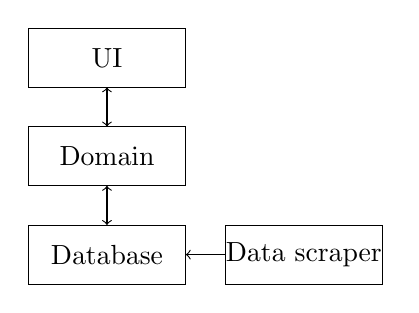
\begin{tikzpicture}
     \draw (0,0) rectangle (2,-0.75) node[pos=0.5] {UI}; 
     \draw[<->] (1,-0.75) -- (1,-1.25) ;
    \draw (0,-1.25) rectangle (2,-2) node[pos=0.5] {Domain}; 
    \draw[<->] (1,-2) -- (1,-2.5);
    \draw (0,-2.5) rectangle (2,-3.25) node[pos=0.5] {Database}; 
    \draw[<-] (2,-2.875) -- (2.5, -2.875);
    \draw (2.5, -2.5) rectangle (4.5, -3.25) node[pos=.5] {Data scraper} ;
  \end{tikzpicture}
  \caption{Architecture of the system}
  \label{fig:layerstructure}
\end{figure}

Regarding the structure of the database we will need to map the user-submitted ingredients
found in recipes to a list of known ingredients. The known list of ingredients, can be
used to query price data. Thus we present the following data structure:

\begin{figure}[H]
  \centering
  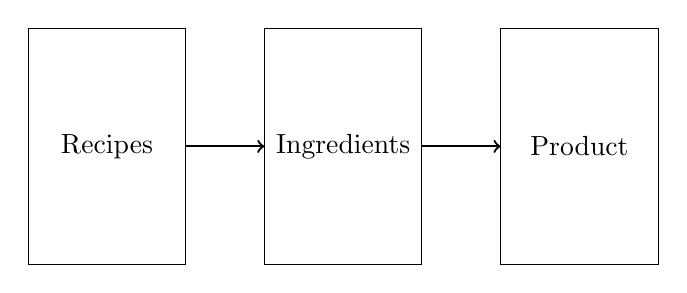
\begin{tikzpicture}
    \draw (0,0) rectangle (2,3) node[pos=.5] {Recipes};
     \draw (3,0) rectangle (5,3)node[pos=.5] {Ingredients};
     \draw[->,thick] (5,1.5) -- (6,1.5);
     \draw[->,thick] (2,1.5) -- (3,1.5);
     \draw (6,0) rectangle (8,3)node[pos=.5] {Product};
  \end{tikzpicture}
  \caption{Overview of the data structure}
\end{figure}

Here we have a list of recipes, the ingredients of these recipes points to a dictionary of
ingredients, which all have unique names. There is no recipes, which ingredients are not
in the dictionary of approved ingredients. Ingredients can have an alias which points to
another ingredient, which is more general.  The dictionary of ingredients, each have an
array of products that they point to. This achieves a separation of recipes and their
prices. 

\subsection{Scraping Data}

We will scraping recipe data from a well-known website called \\\url{www.dk-kogebogen.dk}.
The recipes from this site are user-made, and are thus filled with all sorts of quirks. As
we have using Python we will be using the BeautifulSoup package to help scrap the data from the
site. We want to scrape the table containing the ingredients of the recipe, amounts of the
ingredients and the units of these amounts. We also want the procedure for scraping the
recipe and the title of the recipe. We have identifies that there are in the order of
39027 different recipes numbered in sequential order. As downloading a lot of sites
sequentially is quite slow, it makes sense to do this in parallel. Thus the more
connections we make to the website we would like to scrape, the faster we can get our
results.
\lstset{ %
  backgroundcolor=\color{white},   % choose the background color; you must add \usepackage{color} or \usepackage{xcolor}
  basicstyle=\tiny,        % the size of the fonts that are used for the code
  breakatwhitespace=false,         % sets if automatic breaks should only happen at whitespace
  breaklines=true,                 % sets automatic line breaking
  captionpos=b,                    % sets the caption-position to bottom
  commentstyle=\color{commentsColor}\textit,    % comment style
  deletekeywords={...},            % if you want to delete keywords from the given language
  escapeinside={\%*}{*)},          % if you want to add LaTeX within your code
  extendedchars=true,              % lets you use non-ASCII characters; for 8-bits encodings only, does not work with UTF-8
  frame=tb,	                   	   % adds a frame around the code
  keepspaces=true,                 % keeps spaces in text, useful for keeping indentation of code (possibly needs columns=flexible)
  keywordstyle=\color{keywordsColor}\bfseries,       % keyword style
  language=Python,                 % the language of the code (can be overrided per snippet)
  otherkeywords={*,...},           % if you want to add more keywords to the set
  numbers=left,                    % where to put the line-numbers; possible values are (none, left, right)
  numbersep=5pt,                   % how far the line-numbers are from the code
  numberstyle=\tiny\color{commentsColor}, % the style that is used for the line-numbers
  rulecolor=\color{black},         % if not set, the frame-color may be changed on line-breaks within not-black text (e.g. comments (green here))
  showspaces=false,                % show spaces everywhere adding particular underscores; it overrides 'showstringspaces'
  showstringspaces=false,          % underline spaces within strings only
  showtabs=false,                  % show tabs within strings adding particular underscores
  stepnumber=1,                    % the step between two line-numbers. If it's 1, each line will be numbered
  stringstyle=\color{stringColor}, % string literal style
  tabsize=2,	                   % sets default tabsize to 2 spaces
                  % show the filename of files included with \lstinputlisting; also try caption instead of title
  columns=fixed                    % Using fixed column width (for e.g. nice alignment)
}
\lstinputlisting[language=Python, firstline=89, lastline=97, basicstyle=\footnotesize\ttfamily,
]{../prototype/scrape_recipe_ingredients.py}

With the function \texttt{execute\_get\_in\_parallel} we give it the \texttt{recipe\_id}
to start from and the \texttt{no\_recipes} to scrape. We then pass the name from a
function to be run in parallel. At first a list of urls to crawl is created. Then we take
the \texttt{cpu\_count} of the system to determine the amount threads to spawn. We then
create a \texttt{ThreadPoolExecutor} with \texttt{cpu\_count} threads. In line 6 we then
submit the \texttt{function} and \texttt{url} for a thread from the pool to work on. As
this happens asynchronously, we have no guarantee for when the executors will be done
working. Because of this the executors returns the results in a \texttt{Future} object. We
can iterate over this list of \texttt{Futures} as the executors finish. We then the
results of all the functions are returned in a list for further processing.

\subsection{Sanitizing Data}

\subsection{Getting Prices}

\subsection{Creating Relationships in the Data}

\subsection{User Interface}

\end{document}
